\documentclass[
	%parspace, % Add vertical space between paragraphs
	%noindent, % No indentation of first lines in each paragraph
	%nohyp, % No hypenation of words
	%twoside, % Double sided format
	%draft, % Quicker draft compilation without rendering images
	%final, % Set final to hide todos
]{elteiktdk}[2023/04/10]

% The minted package is also supported for source highlighting
%\usepackage[newfloat]{minted}

% Document's metadata
\title{Vízközeli hulladéklerakók megbízható detektálása multispektrális műholdfelvételek segítségével}
\date{2024}

% Author(s)' metadata
\author{Dénes Botond}
\degree{programtervező informatikus MSc}
\period{2. évfolyam}

% Superivsor(s)' metadata
\supervisor{Cserép Máté}
\affiliation{egyetemi tanársegéd}

% University's metadata
\university{Eötvös Loránd Tudományegyetem}
\faculty{Informatikai Kar}
\department{Programozáselmélet és Szoftvertechnológiai Tanszék}
\city{Budapest}
\logo{elte_cimer_szines}

% Add bibliography file
\addbibresource{elteiktdk.bib}

% The document
\begin{document}

% Set document language
\documentlang{hungarian}
%\documentlang{english}

% List of todos (not in the final document)
%\listoftodos[\todolabel]
%\cleardoublepage

% Cover and title page (mandatory)
\makecover
\cleardoublepage
\maketitle

% Table of contents (mandatory)
\tableofcontents
\cleardoublepage

% Main content
\chapter{Bevezetés}
\label{ch:intro}

\todo{szinkronizálni az absztrakttal}A hulladékszennyezés komoly problémát jelent a természet számára \cite{kibria2023PlasticWaste}. Emiatt számos szervezet mozdul abba az irányba, hogy tisztábbá tegye a bolygónkat. Egy ilyen szervezet a PET Kupa, akik folyómenti hulladékgyűjtéssel foglalkoznak elsősorban Magyarországon, de figyelmük kiterjed a szomszédos országokra is. Az egyik nagy kihívás a szemétgyűjtésben a hulladékkal szennyezett területeknek a hatékony megtalálása. Sok erőforrást igényel a hulladéklerakók megtalálása a folyók mentén, hiszen sokszor járművel kell valakinek végig haladnia egy hosszabb területen, azért, hogy felmérje, hogy hol van hulladék. A folyók árterén elhelyezett hulladékok még nagyobb problémát jelentenek, hiszen dagály idejében a hulladékot elmossa a víz és ez a folyó további szakaszaira lesz szétszórva miközben nagy károkat okoz a folyó élővilágának, illetve szennyezi a folyóvizet \cite{nyberg2023, vanEmmerik2023}. Emiatt szükségünk van olyan eszközökre, melyekkel hamar lehet detektálni a szennyezett területeket, hogy ezeket minél hatékonyabban meglehessen tisztítani. Az ELTE Térinformatikai Labor és a PET Kupa együttműködésében olyan eszközöket fejlesztünk, melyek automatikusan képesek lesznek hulladékot detektálni a folyók mentén.

A dolgozatomban bemutatok egy Random Forest modellt \cite{breiman2001}, mely a kutatólaborban már lefejlesztett modellre épül \cite{magyar2023}. A bemutatott modell javít a korábbi megoldás pontosságán, illetve nagyobb megbízhatósággal találja meg a hulladékot a folyókon és a folyók mentén. A modell eredményei integrálásra kerülnek a Tiszta Tisza webalkalmazásba\footnote{A Tiszta-Tisza webalkalmazás hivatalos weboldala a https://tisztatiszaterkep.hu/ címen található, de a dolgozatban említett fejlesztések jelenleg a https://gis.inf.elte.hu/tiszta-tisza/ oldalon érhetőek el.}, ahol több napon keresztül történő detektálás eredménye lesz összesítve és megjelenítve a felhasználók számára. Ezen felül a dolgozatban tárgyalni fogok más kutatást is, mely a hulladékdetektálás problémájával foglalkozik. Ezen kívül kiegészítem a kutatólabor meglevő szoftveres eszközeit annak érdekében, hogy a laborban zajló munka gördülékenyebb legyen.
\todo[inline,color=blue!50]{Hivatkozd meg a https://tisztatiszaterkep.hu/ oldalt, de említsd meg, hogy a prototípus egyelőre a https://gis.inf.elte.hu/tiszta-tisza/ oldalon érhető el. Ez mehet akár csak lábjegyzetbe. Botond: Rendben, lábjegyzetben megemlítettem.}

A kutatás hozzáadott terméke egy olyan adathalmaz, mely alkalmas más hulladékdetektálási modellek betanítására is. Az adathalmaz elsősorban szárazföldi romániai hulladéklerakókról készített PlanetScope műholdfelvételeket tartalmaz, melyek kézzel voltak annotálva. Az adatok georeferálva vannak, így ezeket könnyen meg lehet vizsgálni, illetve ki lehet egészíteni.

Továbbá bemutatom, hogy milyen módszerekkel próbáltam tovább javítani a modell eredményein. Ilyen módszer például a főkomponens analízis, a képnormalizálás, illetve az évszakokra bontás.

\section{A kutatólabor eddigi eredményei}

A ELTE IK Térinformatikai Kutatólaborában már betanításra került egy Random Forest modell, mely folyómenti hulladék detektálására alkalmas. Az én dolgozatomban, a kutatólabor meglevő tudására építve, továbbfejlesztem ezt a modellt, hogy kevesebb \textit{false positive}-al találja meg a szeméttel szennyezett területeket. Továbbra implementálásra került egy szerveralkalmazás, mely minden nap a Planet szervereiről letölti a legfrissebb felvételeket a vizsgált területekről, és lefuttatja ezeken a képeken az akkori modellt. Ezen felül készült egy webalkalmazás is, ami erről a szerverről letölti az eredményeket, és megjeleníti ezeket, összehasonlításra. A kutatólabor rendelkezik egy asztali alkalmazással is, mellyel hatékonyan elő lehet állítani tanító adatokat. A kutatásom elősegítéséhez ezeket az alkalmazásokat használtam, illetve bővítettem a \ref{ch:application-improvement} fejezetben leírtak szerint.

\section{Kutatási cél}
\label{ch:goals}

A cél az, hogy a kutatás során szerzett modell megbízhatóan detektáljon hulladéklerakókat általánosan folyók mentén. Ehhez a \textit{false positive} arányok minél kisebbek kell legyenek, míg a true positive arányok minél nagyobbak. Ugyanakkor nem jelent ugyanakkora problémát egy \textit{false negative}, mint egy \textit{false positive}, mivel a \textit{false positive} eredmények fölöslegesen rossz irányba küldhetik a folyómentő csapatot. 
A kutatólabor 2023-as cikkében bemutatott modell (továbbiakban meglevő modell vagy régi modell) \cite{magyar2023} egyik problémája a nagy \textit{false positive} arányok voltak. Általában a modellnek leginkább az utak, épületek okoznak problémát. Ez annak köszönhető, hogy a hulladék, a törmelék, az épületek, és a föld nagyon hasonló spektrális értékekkel rendelkeznek a használt sávokon. A modell a pusztazámori hulladéklerakóról, illetve a kiskörei víztárolóról szerzett adatokkal volt betanítva. Ezért egy jó irány több adaton betanítani a modellt, nagy figyelmet fektetve arra, hogy az adathalmaz tartalmazzon bőven utakat, épületeket, és más adatokat, amik hasonlítanak a hulladékra. 

\section{A dolgozat felépítése}
A \ref{ch:related_research}. fejezetben bemutatásra kerülnek a hulladékdetektálás témáját feldolgozó kutatások, illetve bemutatom azokat a technikai és számolási eszközöket, melyek lényeges szerepet vállalnak a kutatásomban.
A \ref{ch:training}. fejezetben részletezem a Random Forest modell betanításához előállított adatokat, a modell betanítási paramétereit, illetve megvizsgálok különböző adatfeldolgozási módszereket, ilyen például a főkomponens analízis, képnormalizálás, vízmaszkolás, azzal a céllal, hogy tovább javítsak a modell teljesítményén. A \ref{ch:verification}. fejezetben tárgyalom a modell tesztelésének és validálásának módját, illetve a tesztadatok megválasztásának módját, motivációját. A \ref{ch:impl}. fejezetben bemutatom a kutatást lényegesen előresegítő szoftveres fejlesztéseket, azt, hogy a kutatás eddigi eredményei miként vannak integrálva a Tiszta-Tisza alkalmazásba. A \ref{ch:sum}. fejezetben összefoglalom a kutatás eredményeit, és ezek alapján tárgyalom a kutatás további lehetséges haladásait. 
\cleardoublepage

\chapter{Elemzés és tervezés}
\label{ch:spec}

\section{Kutatási cél}
\label{ch:goals}

A cél az, hogy a kutatás során szerzett modell megbízhatóan detektáljon hulladéklerakókat általánosan folyók mentén. Ehhez a false positive arányok minél kisebbek kell legyenek, míg a true positive arányok minél nagyobbak. Ugyanakkor nem jelent ugyanakkora problémát egy false negative, mint egy false positive, mivel a false positive eredmények fölöslegesen rossz irányba küldhetik a folyómentő csapatot. 
A kutatólabor 2023-as cikkjében bemutatott modell (továbbiakban meglevő modell) egyik problémája a nagy false positive arányok voltak. A modell a pusztazámori hulladéklerakóról, illetve a kiskörei víztárolóról szerzett adatokkal volt betanítva. Ezért érdemes első körben egy nagyobb adathalmazzal betanítani a modellt.

\section{Műhold specifikációk}

Az új Random Forest modell a PlanetScope műholdakra van specializálva, azon belül is a legújabb PSB.SD szenzorokra. A modell a Vörös (Red), Kék (Blue), Zöld (Green), és a közeli infravörös (NIR) sávokat használja. A PlanetScope műholdak körülbelül 3 méter/pixel felbontással rendelkeznek \cite{planetsensors2024}.

\section{Használt indexek}

A kutatás során felhasználom a kutatólaborban már számolt indexeket. Pontosabban a Plastic Index (\ref{eq:pi} képlet), Normalized Difference Water Index (\ref{eq:ndwi} képlet), Normalized Difference Vegetation Index (\ref{eq:ndvi} képlet), Reversed Normalized Difference Vegetation Index (\ref{eq:rndvi} képlet), Simple Ratio (\ref{eq:sr} képlet) indexek kerülnek használatra \cite{Themistocleous2020, magyar2023}.

\begin{equation}\label{eq:pi}
    Plastic Index (PI) = \frac{NIR}{NIR + Red}
\end{equation}

\begin{equation}\label{eq:ndwi}
    Normalized Difference Water Index (NDWI) = \frac{Green - NIR}{Green + NIR}
\end{equation}

\begin{equation}\label{eq:ndvi}
    Normalized Difference Vegetation Index (NDVI) = \frac{NIR - Red}{NIR + Red}
\end{equation}

\begin{equation}\label{eq:rndvi}
    Reversed Normalized Difference Vegetation Index (NDVI) = \frac{Red - NIR}{Red + NIR}
\end{equation}

\begin{equation}\label{eq:sr}
    Simple Ratio (SR) = \frac{NIR}{Red}
\end{equation}


\cleardoublepage

\chapter{Betanítás}
\label{ch:training}

\section{Tanítóadatok}

A betanításhoz 29 romániai hulladéklerakó és közvetlen környezete került a tanítóadatok közé, illetve a Kiskörei víztároló is. A víztároló már vizsgálva volt \cite{magyar2023}-ban, és alkalmas úszó hulladéksziget detektálására, tekintve arra, hogy a felgyült faágak között nagy koncentrációban jelenik meg műanyag-alapú hulladék. A \ref{fig:kiskore-waste} ábrán látható, hogy miként gyűl össze a hulladék a víztárolónál. A romániai hulladéklerakókat egy helyi weboldalon lehet megtalálni, a hozzájuk tartozó koordinátákkal együtt \cite{wasteromania2019}. Az ott bemutatott 46 hulladéklerakó közül 29 volt alkalmas tanításra: sok hulladéklerakó be lett tömve, vagy föld alatt működik. Minden hulladéklerakóhoz letöltöttem egy-egy nyári+tavaszi, téli és őszi multispektrális műholdképet, melyeket kézzel annotáltam. A nyári és tavaszi képeket azért vontam egybe, mivel ezek hulladékdetektálás szempontjából hasonló adatokat eredményeztek. A tanítóadatok pixelenként vannak előállítva, így a végső adathalmaz 27 millió tanítóadatból (pixelből) áll. Minden pixelhez hozzá van rendelve a vörös, kék, zöld, közeli infravörös sáv, illetve a "PI", "NDWI", "NDVI", "RNDVI", "SR" indexek. Ezen felül minden pixel címkézve van a \ref{tab:waste-detection-labels} táblázatban leírtak szerint. Nagyon fontos, hogy minél pontosabban meg lehessen állapítani, hogy a hulladéklerakókon mely területeken található hulladék, hiszen sok hulladéklerakón törmeléket is tárolnak, ezt általában egy külön területen. Emiatt a tanítóadatokat a következő módszerrel állítottam elő: Megvizsgáltam Google Maps segítségével \cite{googlemaps2024}, hogy az adott hulladéklerakónál hol tárolnak törmeléket és hol tárolnak műanyag alapú hulladékot. A Google Maps légi felvételei elég magas felbontással rendelkeznek ahhoz, hogy általában szemmel meglehessen különböztetni a műanyag alapú hulladékot a törmeléktől. A \ref{fig:waste-vs-debris} ábrából látható, hogy míg a törmelék inkább fehér színt tartalmaz, addig a műanyag alapú hulladék picit vörösebb, tekintve arra, hogy a műanyag sokszor színezve van. Emellett, a hulladéklerakókat nagyon konzervatívan jelöltem ki: csak akkor jelöltem be egy területet, mint hulladékos terület, ha a felvételből egyértelmű volt, hogy az adott terület műanyag alapú hulladékkal szennyezett. Természetesen, helyi terepvizsgálattal, illetve magasabb felbontású felvételek készítésével pontosabb adatokat lehetne előállítani. 

\begin{figure}[H]
	\centering
	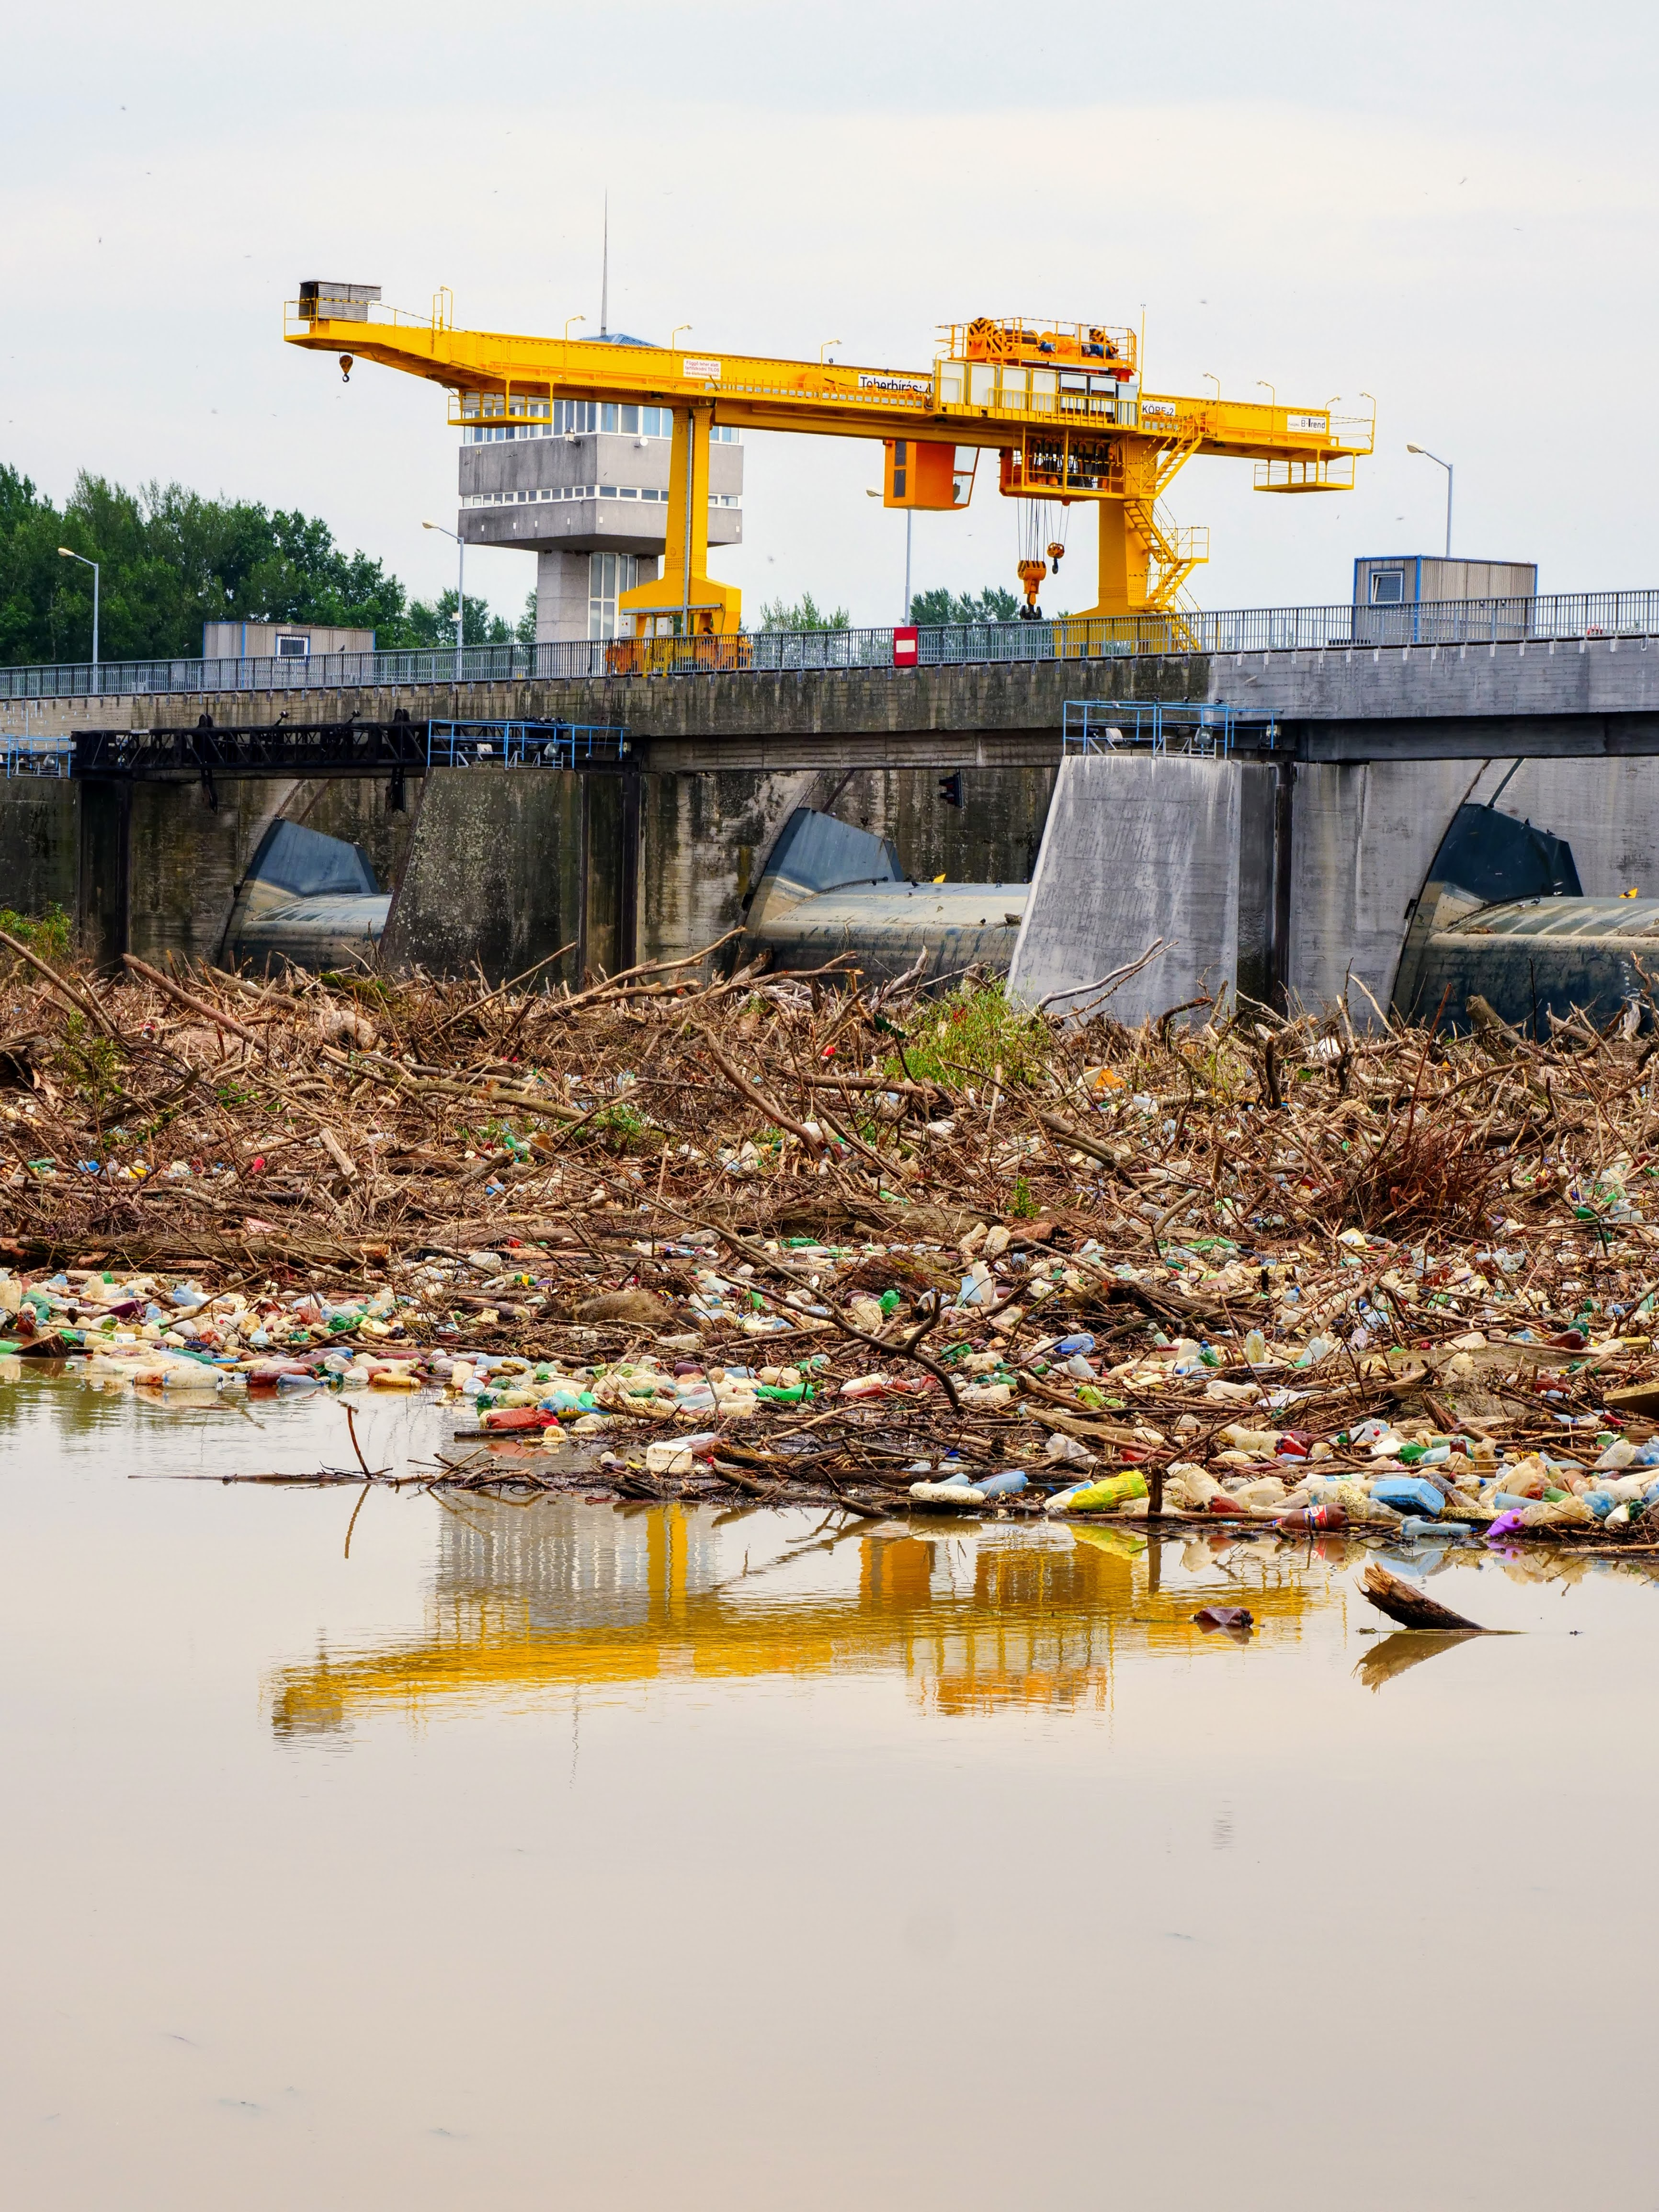
\includegraphics[width=0.6\textwidth,frame]{kiskore-garbage}
	\caption{A kiskörei víztároló hulladéktorlasza \cite{petkupa2024}}
    \label{fig:kiskore-waste}
\end{figure}

\begin{table}[H]
	\centering
	\begin{tabular}{ | p{0.1\textwidth} | p{0.2\textwidth} | p{0.6\textwidth} | }
		\hline
		\textbf{Címke azonosító} & \textbf{Címke neve} & \textbf{Címke magyarázat} \\
		\hline \hline
		\emph{100} & Hulladék & Azon területek, melyeken hulladék van. \\
		\hline
		\emph{200} & Víz & olyan területek, melyeken kizárólag víz van, általában folyók. \\
		\hline
		\emph{300} & Legelők/Erdők & Zöld övezetből álló vad területek. Ezek lehetnek fák lombjai vagy füves zónák. \\
		\hline
        \emph{400} & Mezők & Olyan földes területek, melyek meg vannak művelve, illetve ahol mezőgazdasági növények találhatóak, például gabonafélék. \\
		\hline
        \emph{500} & Ismeretlen & Olyan területek, melyek a korábbi kategóriákba nem sorolhatók bele. Ilyenek az épületek, aszfaltozott utak, háztetők, mezei utak. \\
		\hline
	\end{tabular}
	\caption{A tanítóadatok címkéi}
	\label{tab:waste-detection-labels}
\end{table}

\begin{figure}[H]
	\centering
	\subcaptionbox{Műanyag alapú hulladék}{
		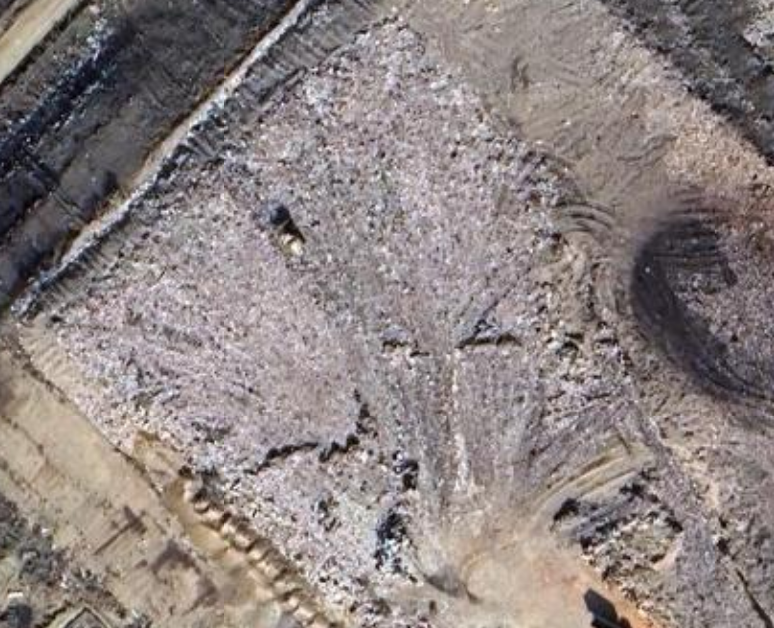
\includegraphics[width=0.45\linewidth]{waste}}
	\hspace{5pt}
	\subcaptionbox{Törmelék}{
		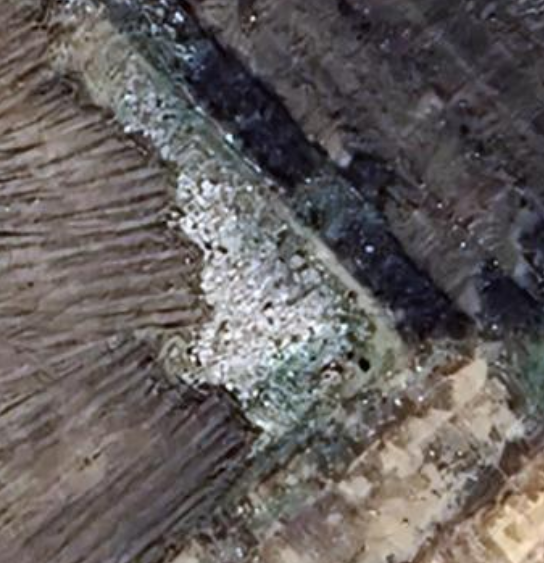
\includegraphics[width=0.45\linewidth]{debris}}
	\caption{A műanyag alapú hulladék, törmelék mellé helyezve. Forrás: Google Maps}
	\label{fig:waste-vs-debris}
\end{figure}



\section{Tanítási paraméterek}
\label{ch:teaching-params}

A Random Forest betanításához a Scikit-Learn Python csomagot használtam \cite{scikit-learn}. A nagy adathalmaz miatt a Random Forest modell is nagyon nagy lett (körülbelül 14GB), ami egy nehezen kezelhető méret, így érdemes módosítani a modell paraméterein, hogy ez kisebb méretű legyen. A legjobb eredményeket azzal értem el, hogy a Random Forest fák méretét 20 mélységűre limitáltam. Ennek köszönhetően a model méretét 2GB-ra tudtam csökkenteni, és a \ref{fig:fullsize-vs-reduced} ábrából látható, hogy a csökkentett modellben enyhén megnő a hulladékra vonatkozó false-negative ráta, míg a false positive arány nem nő, de cserében egy kezelhető méretű modellt kapok.

\begin{figure}[H]
	\centering
  \subcaptionbox{A klasszifikálandó felvétel}{
		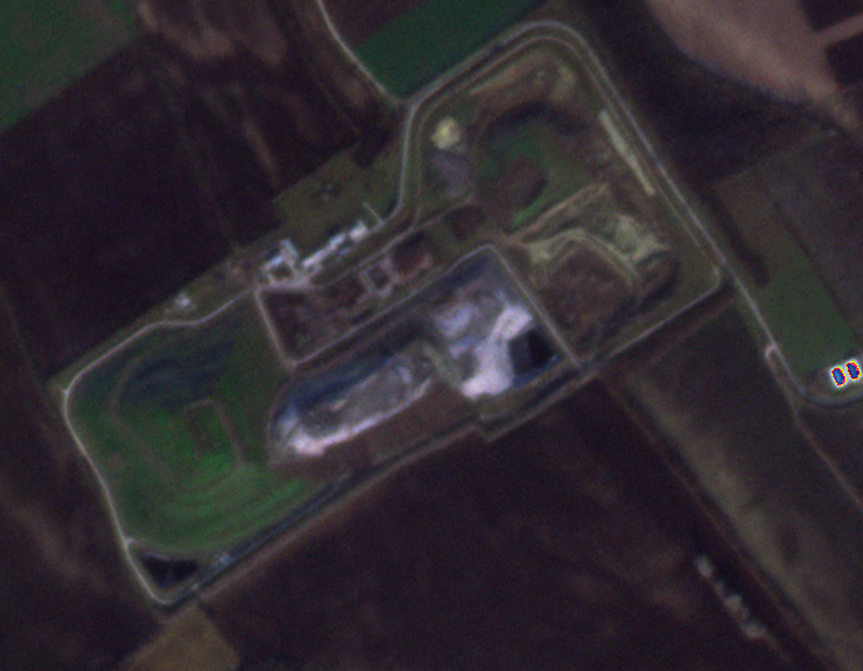
\includegraphics[width=0.45\linewidth]{original-pusztazamor}}
	\hspace{5pt}
	\subcaptionbox{Teljes méretű modell}{
		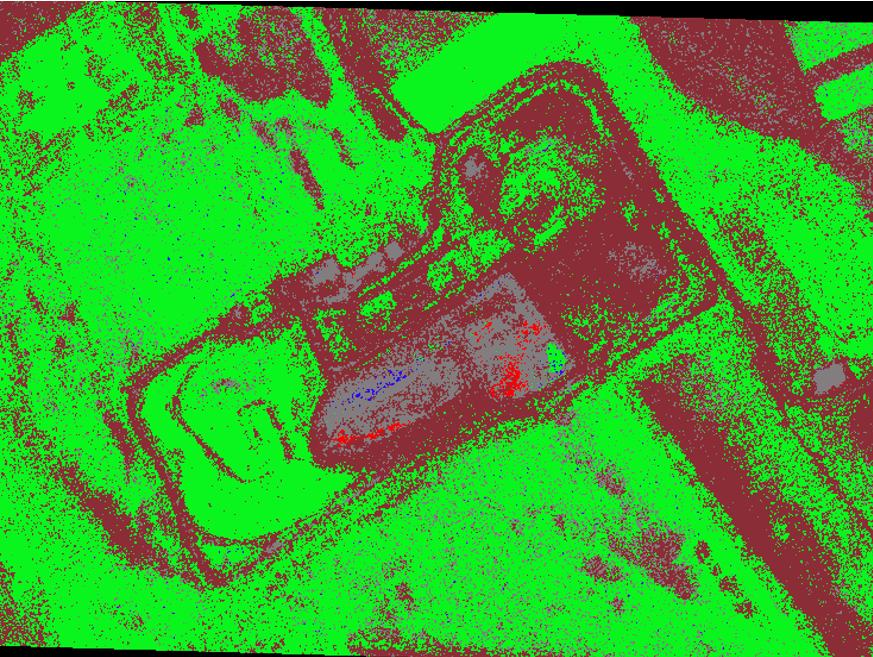
\includegraphics[width=0.45\linewidth]{fullsized}}
	\hspace{5pt}
	\subcaptionbox{Csökkentett modell}{
		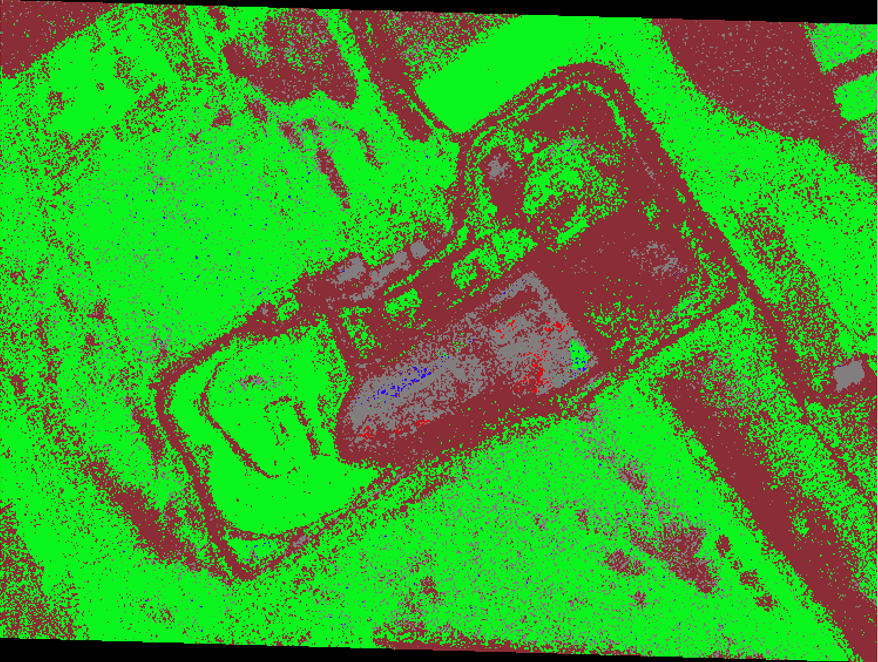
\includegraphics[width=0.45\linewidth]{reduced}}
	\caption{A csökkentett modell hasonlóan teljesít a teljes méretű modellhez}
	\label{fig:fullsize-vs-reduced}
\end{figure}

Továbbiakban felmerült az a probléma is, hogy a tanítóadatok nagyon aránytalanok: A \ref{fig:unbalanced-data} ábrából látható, hogy nagyságrendekkel kevesebb adattal rendelkeztünk hulladékról, mint az összes többi adatról. Emiatt a modell nagyon sok false-negatívot termelt. Ennek korrigálására súlyokat alkalmaztam a tanítóadatokra. A súlyok kiszámolásához az összes címkére a \ref{eq:weights} képletet használtam.

\pgfplotstableread[row sep=\\,col sep=&]{
    label           & value     \\
    Hulladék        & 29513     \\
    Víz             & 926356    \\
    Legelők/Erdők   & 12573615  \\
    Mezők           & 8043948   \\
    Ismeretlen      & 5669416   \\
}\datacounts

\begin{figure}
    \begin{tikzpicture}
        \begin{axis}[
                ybar,
                ymode = log,
                bar width=1cm,
                width=\textwidth,
                height=0.5\textwidth,
                symbolic x coords={Hulladék,Víz,Legelők/Erdők,Mezők,Ismeretlen},
                xtick=data,
            ]
            \addplot table[x=label,y=value]{\datacounts};
        \end{axis}
    \end{tikzpicture}
    \caption{Az adatok közötti aránytalanság, logaritmikus skálázással}
    \label{fig:unbalanced-data}
\end{figure}

\begin{equation}\label{eq:weights}
    c\acute{\imath}mke \ s\acute{u}lya=\frac{adathalmaz \ m\acute{e}rete}{c\acute{\imath}mke \ darabsz\acute{a}ma}
\end{equation}

\section{Felvételek normalizálása}

Az egyik gyakori probléma gépi tanulásban az, hogy ha elég nagy eltérések vannak a felvételek között, például időjárás miatt, akkor a modell hajlandó félreosztályozni egyes területeket. Illetve, a műholdak, amikkel készülnek a felvételek idővel újabb műszereket kapnak, amik eltéréseket termelhetnek a felvételeken. Ennek fényében időben is lehetnek lényeges eltérések a felvételek között. Ennek korrigálára érdemes megvizsgálni a műholdfelvételek normalizálását. A normalizálás egy referencia kép szerint történik: kiválasztok egy referencia felvételt egy adott területről és időszakról (nyár, tél), és az összes többi felvételt arról a területről és időszakról erre a felvételre normalizálom. Így a nagymértékű eltérések csökkentve lesznek a modell számára, és várhatóan jobban fogja osztályozni a felvételeket, amik különböző körülmények között voltak előállítva. A normalizáló algoritmust az ELTE IK térinformatikai laboron belül fejlesztette az egyik kollégám.
A normalizált felvételekhez külön kell egy modellt betanítani. Így a teszthalmazban minden területhez és minden évszakhoz kiválasztottam egy-egy felvételt, mint referencia kép. Ezután minden műholdképet normalizáltam a referenciához. A módszer eredményeit a \ref{ch:normalization-test} fejezetben részletezem.

\section{Főkomponens analízis (PCA)}
\label{ch:pca-methodology}

A modell méretének a csökkentésére megvizsgáltam a főkomponens analízis (PCA) alkalmazását is \cite{pca2010}. A főkomponens analízis a gépi tanulásban egy szélesen elterjedt módszer.  A módszer lényege az, hogy egy többdimenziós adathalmazból kivonja a legfontosabb információkat egy alacsonyabb dimenziószámú adathalmazba. Ezeket nevezzük főkomponenseknek. A főkomponensek korrelálatlanok, vagyis a korrelációs mátrixuknak a főátlóján helyezkednek el, illetve a megfigyelési egységek varianciájának a nagy részét az első pár főkomponensben tároljuk \cite{elek2011}. Azt, hogy hány főkomponenst szeretnénk megtartani, empirikus módon meghatározhatjuk annak függvényében, hogy mekkora mértékben szeretnénk megtartani az eredeti adathalmaz varianciáját. A \ref{fig:pca-variance} ábrán látható, hogy ennek az adathalmaznak az esetében ha 90\%-át szeretném megtartani a varianciának, akkor elég az első három főkomponenst megválasztanom. Így a továbbiakban, minden PCA alkalmazáskor az első három főkomponens kiválasztása értendő.

\pgfplotstableread[row sep=\\,col sep=&]{
    label           & value     \\
    PC1        & 6.673e+01     \\
    PC2             & 2.239e+01    \\
    PC3   & 6.859e+00  \\
    PC4           & 2.032e+00   \\
    PC5     & 1.501e+00    \\
    PC6 & 4.057e-01    \\
    PC7 & 8.222e-02    \\
    PC8 & 5.806e-13    \\
    PC9 & -9.228e-27    \\
}\varianceretention

\begin{figure}
    \begin{tikzpicture}
        \begin{axis}[
                ybar,
                ylabel=megtartott variancia(\%),
                bar width=1cm,
                width=\textwidth,
                height=0.5\textwidth,
                symbolic x coords={PC1,PC2,PC3,PC4,PC5,PC6,PC7,PC8,PC9},
                xtick=data,
            ]
            \addplot table[x=label,y=value]{\varianceretention};
        \end{axis}
    \end{tikzpicture}
    \caption{A főkomponensek varianciája a tanítóhalmazon. 90\% variancia megtartásának érdekében elég az első három főkomponenst kiválasztani}
    \label{fig:pca-variance}
\end{figure}

A PCA használatának a motivációja az volt, hogy a bemeneti adatok dimenziószámának a csökkentésével csökkenni fog a modell mérete, de érdekes módon a modell mérete nem csökkent a dimenziószám csökkentésével, helyette lényegesen megnőtt. Ezt az is tükrözi, hogy megnőtt átlagosan a Random Forest döntési fáinak a mérete, minél kevesebb dimenziószámú adatot kapott. A \ref{tab:increase-in-model-size} táblázatból látható, hogy különböző főkomponenseknél mekkora volt átlagban a fák mérete az adatok dimenziószámának függvényében. További vizsgálatok után kiderült, hogy hogyha kevesebb dimenziójú adatot adtam a modellnek, akkor a mérete lényegesen megnőtt. 

Ezen felül az is célja volt a PCA alkalmazásának, hogy a kiszámolt indexek információit megtartva, alacsonyabb dimenziószám segítségével a Random Forest modell hatékonyabban fogja majd feldolgozni a műholdfelvételeket. \cite{Howley2005} megmutatja, hogy egyes modelleken jobb klasszifikációt tudtak elérni több spektrális sávból álló adat esetén. Ennek az az oka, hogy ha igen sok a korreláció a különböző dimenziók között, akkor a modell rátanulhat a zajra. Mivel a modell által használt indexek között sok a korreláció, érdemes megvizsgálni a PCA-t olyan szempontból is, hogy esetleg javít-e a klasszifikációs eredményeken. 

\begin{table}[H]
	\centering
	\begin{tabular}{ | p{0.3\textwidth} | p{0.3\textwidth} | }
		\hline
		\textbf{Főkomponensek száma} & \textbf{Fák méretének mediánja} \\
		\hline \hline
		Főkomponensek nélkül (9 dimenzió) & 71.5 \\
		\hline
    5 főkomponens & 71 \\
		\hline
		4 főkomponens & 73\\
		\hline
    3 főkomponens & 85 \\
    \hline
	\end{tabular}
	\caption{A döntési fák méretének a mediánja nem csökkent, amint a főkomponensek száma csökkent, cserében 3 főkomponensnél már nőtt.}
	\label{tab:increase-in-model-size}
\end{table}

A PCA alkalmazása a Random Forestre a következő lépésekből áll:
\begin{enumerate}
	\item A tanítóadatok standard skálázása a \ref{eq:standard-scaling} képlet szerint.
	\item A főkomponens analízis alkalmazása a tanítóadatokra.
	\item A Random Forest modell betanítása a tanítóadatokon.
\end{enumerate}
A főkomponens analízis folyamatának a geometriai jelentését a \ref{fig:elek-pca} ábra illusztrálja.

\begin{equation}\label{eq:standard-scaling}
  f(x) = \frac{x - Average}{Standard \ Deviation}
\end{equation}

\begin{figure}[H]
	\centering
	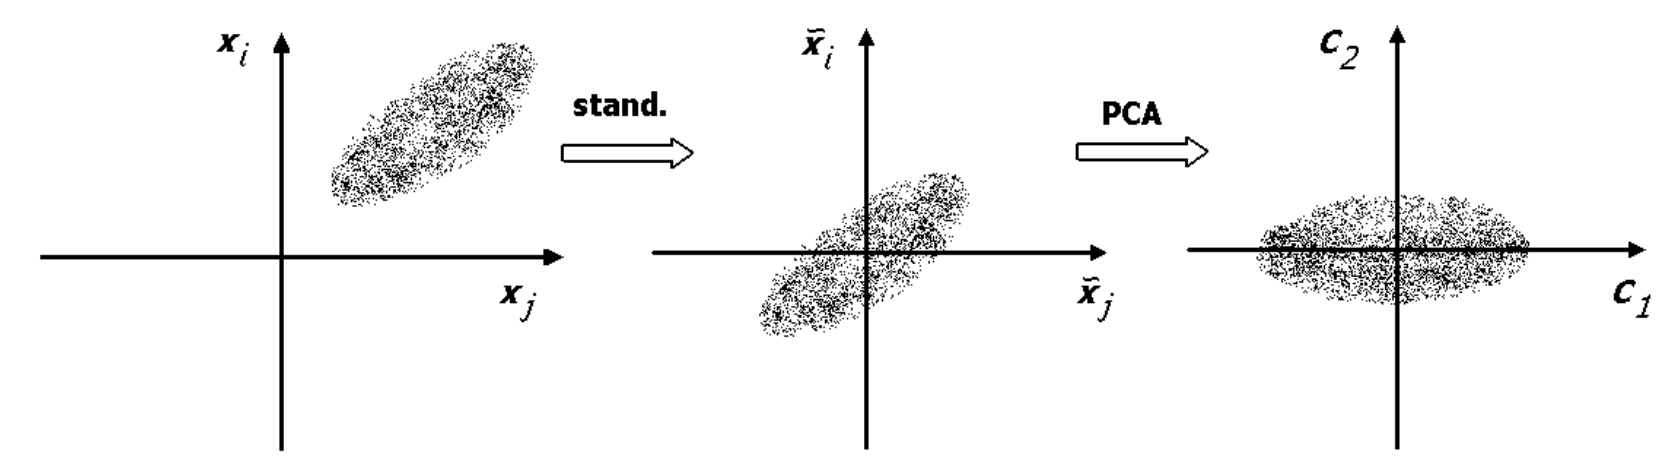
\includegraphics[width=\textwidth,frame]{elek_pca}
	\caption{A főkomponens analízis geometriai jelentése: a standardizálás 0 várható értékűvé és
  1 empirikus szórásúvá teszi a változókat, vagyis a pontfelhőt betolja az origóba,
  majd elforgatja a legnagyobb variancia irányába, ami az első főkomponens \cite{elek2011}}
    \label{fig:elek-pca}
\end{figure}

A modell tesztelésére is ugyanezeket a lépéseket kell elvégezni. A főkomponens analízis használásához a scikit-learn \cite{scikit-learn} Python programcsomagot használtam. A főkomponens analízissel betanított modellt a \ref{ch:teaching-params} fejezetben leírtak szerint paramétereztem. A \ref{ch:pca-performance} fejezetben részletezem a főkomponens analízissel tanított modell teljesítményét.

\section{Nyári és téli adatokra való lebontás}

Alapértelmezetten a nyári és téli adatok között lényeges különbség tud lenni távérzékelés szempontból Közép-Európa területén: a téli időszakokban gyérebb a vegetáció, ködösebb a levegő, illetve a nap sem süt ugyanabból a szögből. Ez befolyásolhatja a modell pontosságát is az adott időszakokban. A nyári időszakot márciustól októberig tartó időszakként definiáltam, és a téli időszak pedig novembertől februárig tart. Az időszakok aszerint vannak megválasztva, hogy mikor leveleznek ki, illetve hullatják ki a leveleiket a fák. Valóban, az októberi időszakban már inkább sárgásak lesznek a levelek, de az októberi tanítóhalmaz mérete önmagában igen kicsi érdemi tanításra. A \ref{fig:winter-vs-summer} ábrából látható, hogy főleg a közeli infravörös (NIR) sávokon nagy eltérések vannak a nyári és téli felvételek között. Ennek fényében betanítottam külön egy nyári és egy téli modellt, melyek teljesítményét a \ref{ch:summer-winter-models} fejezetben részletezem.

\begin{figure}
    \begin{tikzpicture}
        \begin{axis}
          [
          title={Téli felvételek értékei},
          boxplot/draw direction=y,
          ytick={0,2000,4000,6000},
          ymax={8000},
          xtick={1,2,3,4},
          xticklabels={Kék, Zöld, Piros, NIR},
          ]
          \addplot+[
          boxplot prepared={
            median=428,
            upper quartile=563,
            lower quartile=315,
            upper whisker=935,
            lower whisker=44
          },
          ] coordinates {};
          \addplot+[
          boxplot prepared={
            median=530,
            upper quartile=695,
            lower quartile=385,
            upper whisker=1160,
            lower whisker=1
          },
          ] coordinates {};
          \addplot+[
          boxplot prepared={
            median=674,
            upper quartile=923,
            lower quartile=497,
            upper whisker=1562,
            lower whisker=22
          },
          ] coordinates {};
          \addplot+[
            boxplot prepared={
              median=1629,
              upper quartile=2067,
              lower quartile=1273,
              upper whisker=3258,
              lower whisker=82
          },
          ] coordinates {};
        \end{axis}
      \end{tikzpicture}
      \begin{tikzpicture}
        \begin{axis}
          [
          title={Nyári felvételek értékei},
          boxplot/draw direction=y,
          ytick={0,2000,4000,6000},
          ymax={8000},
          yticklabel=\empty,
          xtick={1,2,3,4},
          xticklabels={Kék, Zöld, Piros, NIR},
          ]
          \addplot+[
          boxplot prepared={
            median=360,
            upper quartile=638,
            lower quartile=214,
            upper whisker=1274,
            lower whisker=1
          },
          ] coordinates {};
          \addplot+[
          boxplot prepared={
            median=578,
            upper quartile=862,
            lower quartile=415,
            upper whisker=1532,
            lower whisker=1
          },
          ] coordinates {};
          \addplot+[
          boxplot prepared={
            median=579,
            upper quartile=1058,
            lower quartile=270,
            upper whisker=2240,
            lower whisker=1
          },
          ] coordinates {};
          \addplot+[
            boxplot prepared={
              median=2850,
              upper quartile=3830,
              lower quartile=2103,
              upper whisker=6420,
              lower whisker=1
          },
          ] coordinates {};
        \end{axis}
      \end{tikzpicture}
    \caption{Nyári és téli adatok összehasonlítása}
    \label{fig:winter-vs-summer}
\end{figure}
\cleardoublepage

\chapter {Tesztelés}
\label{ch:testing}

\section{A teszthalmaz}
\label{ch:test-set}

A teszthalmaz három drinai felvételből áll, amin kézzel annotáltam a hulladékkal szennyezett területeket. Ez a terület egyben egy szárazföldi hulladéklerakót \ref{fig:drina-deposit}, illetve egy vízfelszíni hulladékszigetet is tartalmaz, így alkalmas mindkét detektálásnak a tesztelésére. A \ref{fig:drina-floating-waste} ábrából látható, hogy Drinán úgy fogják meg az úszó műanyag-alapú hulladékot, hogy egy zsinorra ráhúznak üres hordókat, melyek a víz felszínén lebegnek. Így, minden, ami elég könnyű ahhoz, hogy a folyó felszínen ússzon (műanyagpalackok, kisebb fadarabok) megakad a hordók mögött, míg például nagyobb fadarabok, vagy más, nehezebb uszadékok a zsinor alatt elúsznak. Így a folyó felszínén kialakuló sziget nagy koncentrációban tartalmaz műanyag alapú hulladékot, tehát alkalmas arra, hogy a modellt ezen validáljam vízfelszíni hulladékdetektáláshoz. Ráadásul erről a területről nem készültek tesztadatok ebben a kutatásban, így a modell teljesítménye az itteni felvételeken jól tesztelhető. A \ref{fig:old-vs-new} ábrából látható egy-egy vizuális összehasonlítás a régi és az új modell klasszifikációja között a teszthalmaz egyik felvételén. Látszik ezen a példán, hogy az új modell több false negative-ot termel főleg a hulladéksziget körül, de ugyanakkor lényegesen lecsökkenti a false positive-ok arányát a régi modellhez képest. Ráadásul a folyó mellett található hulladéklerakót is megtalálja az új modell, míg a régi modell nem találja meg, ellenben a lerakó környékét és az utakat, épületeket gyakran hulladéknak detektálja. Ez egy fontos eredmény, hiszen amint a \ref{ch:goals} fejezetben is tárgyaltam, célja ennek a kutatásnak, hogy csökkentsem a modell false positive arányait, miközben továbbra is meg tudja találni a hulladéklerakókat, illetve hulladékszigeteket.

\begin{figure}[H]
	\centering
	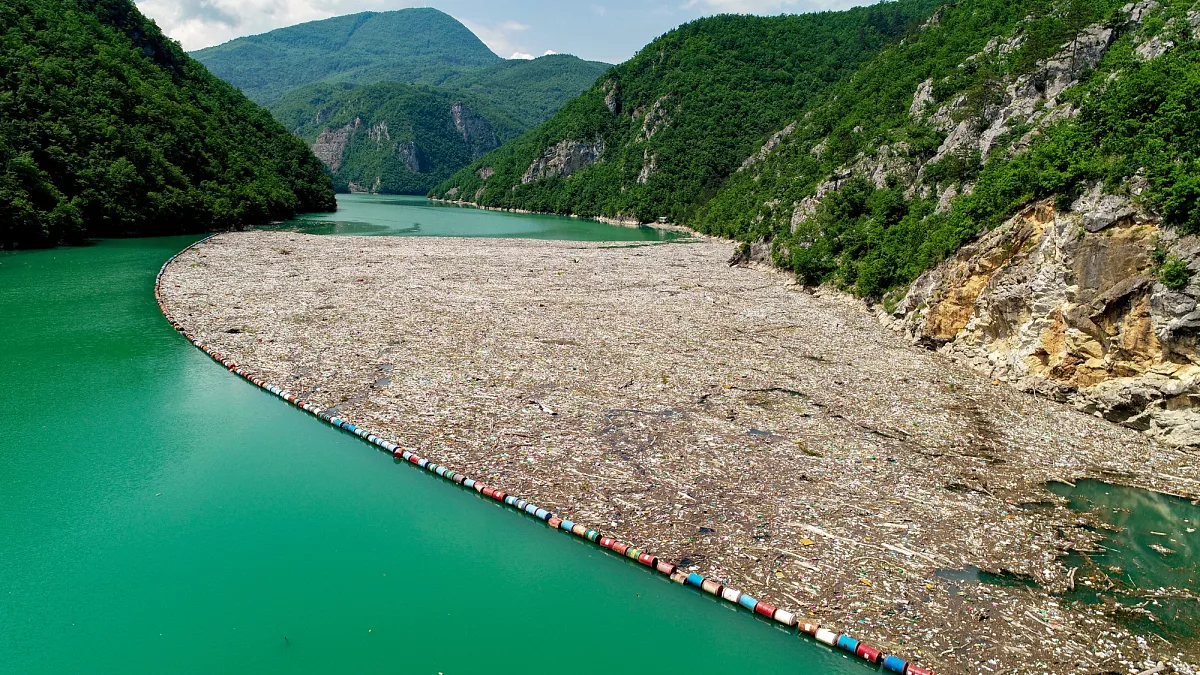
\includegraphics[width=0.6\textwidth,frame]{drina_waste}
	\caption{A drinai hulladéksziget. Egy lebegő zsinor fogja meg a műanyagpalackokat \cite{euronews2024}}
    \label{fig:drina-floating-waste}
\end{figure}

\begin{figure}[H]
	\centering
	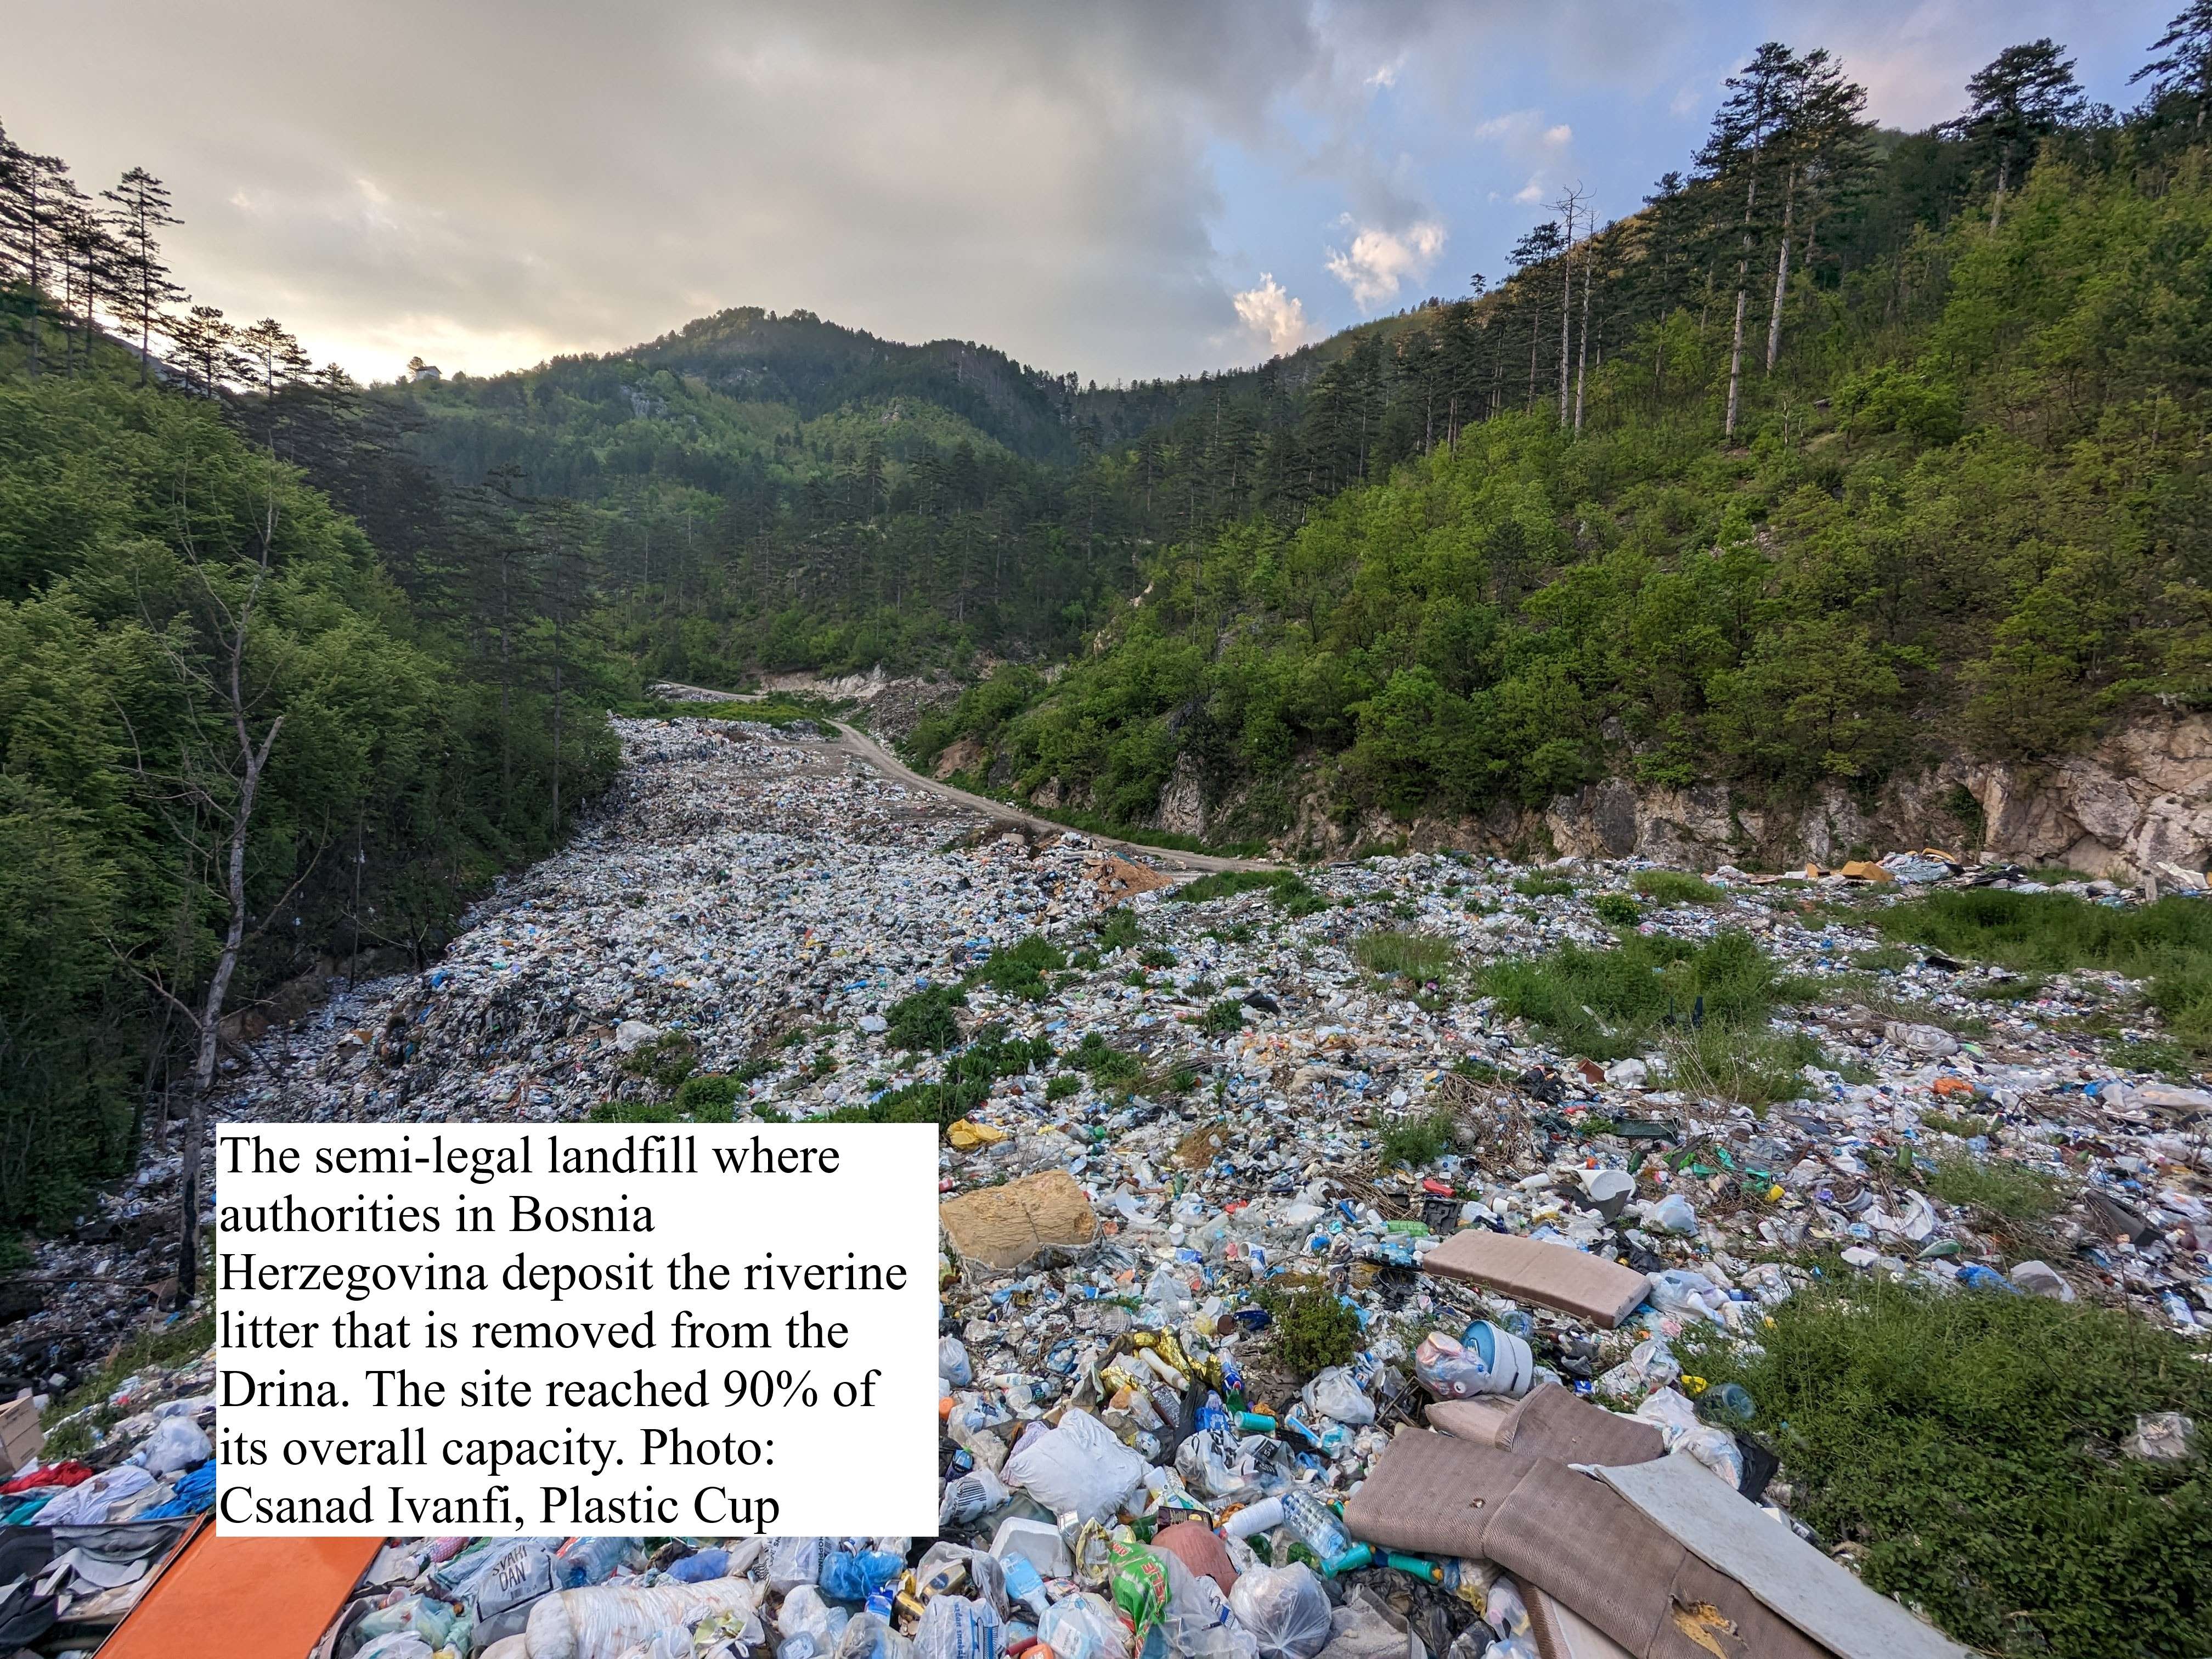
\includegraphics[width=0.6\textwidth,frame]{drina_deposit}
	\caption{A Drina melletti féllegális szemétlerakó \cite{petkupa2024}}
    \label{fig:drina-deposit}
\end{figure}

\begin{figure}[H]
	\centering
  \subcaptionbox{A teszthalmaz kézi annotációja}{
		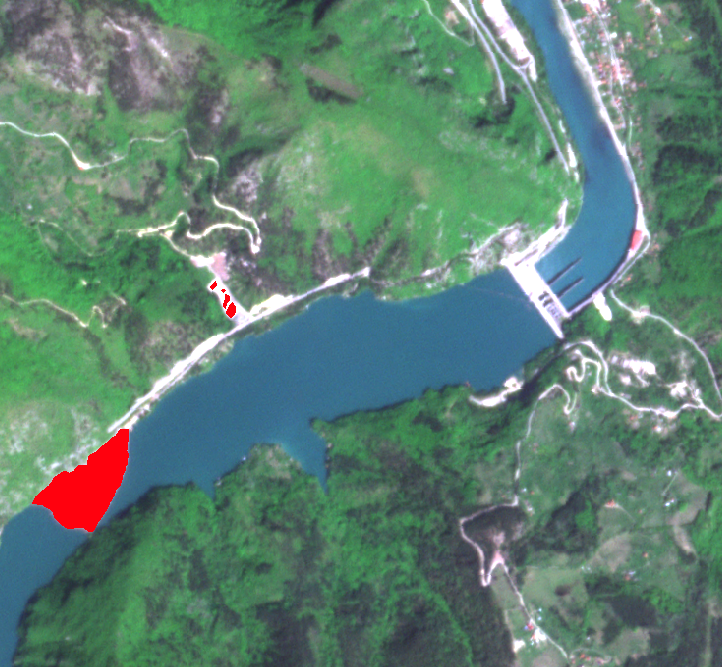
\includegraphics[width=0.45\linewidth]{drina-test}}
	\hspace{5pt}
	\subcaptionbox{A teszthalmaz annotációja a régi modellel}{
		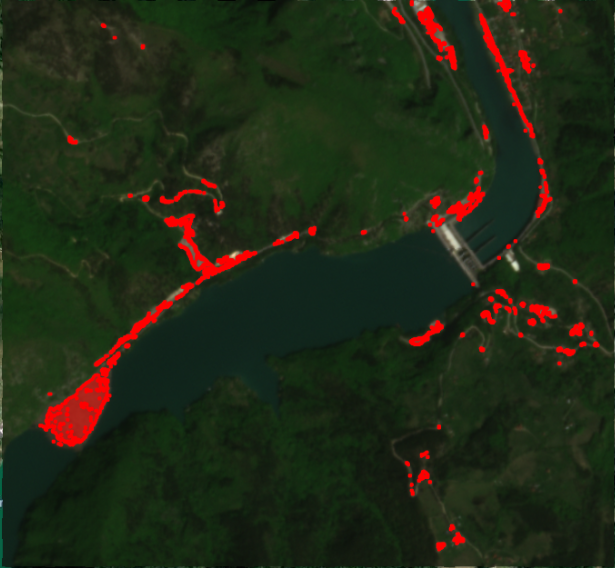
\includegraphics[width=0.45\linewidth]{drina-old}}
	\hspace{5pt}
	\subcaptionbox{A teszthalmaz annotációja az új modellel}{
		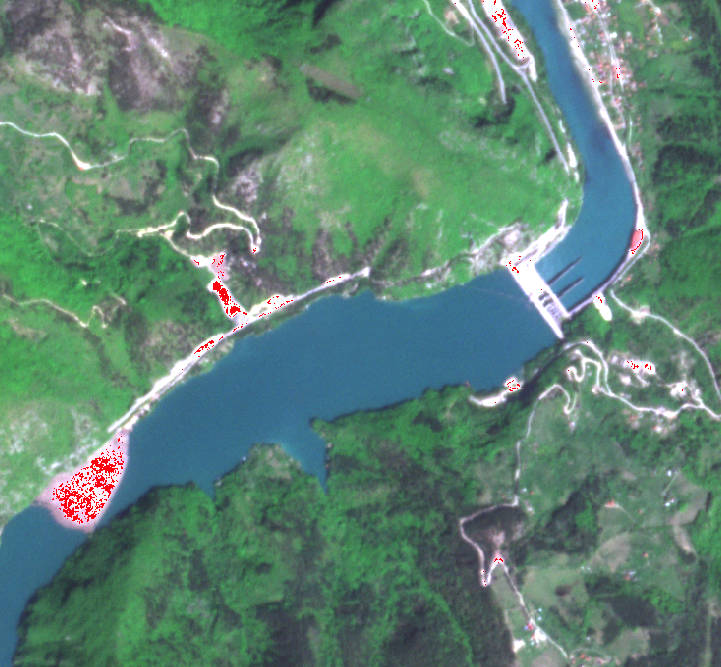
\includegraphics[width=0.45\linewidth]{drina-new}}
	\caption{Az új modell összehasonlítása a régi modellel az egyik Drinai teszt felvételen. Felvétel dátuma: 2023-05-07}
	\label{fig:old-vs-new}
\end{figure}

\section{Teljesítmény mérése}

A teszthalmaz eredményekeit a "Confusion Matrix" módszerével értékeltem ki \cite{CONGALTON199135}. Ezután ezeket az értékeket arra használtam, hogy a "Comission rate" (\ref{eq:comission-rate} képlet), "Omission rate" (\ref{eq:omission-rate} képlet), "Match rate" (\ref{eq:match-rate} képlet), illetve "Extraction rate" (\ref{eq:extraction-rate} képlet) értékeket számítsam ki \cite{Fekete2021}.

\begin{equation}\label{eq:comission-rate}
    Comission \ rate = \frac{N_{com}}{N_{ref}}
\end{equation}

\begin{equation}\label{eq:omission-rate}
    Omission \ rate = \frac{N_{om}}{N_{ext}}
\end{equation}

\begin{equation}\label{eq:match-rate}
    Match \ rate = \frac{N_{match}}{N_{ref}}
\end{equation}

\begin{equation}\label{eq:extraction-rate}
    Extraction \ rate = \frac{N_{ext}}{N_{ref}}
\end{equation}

$N_{com}$, $N_{om}$, $N_{match}$, $N_{ext}$, $N_{ref}$, rendre a false positive, false negative (A mátrix mellékátlói), true positive (A mátrix főátlója), a modell által detektált pozitív, illetve a referencia adatokban található positív értékek. Összehasonlítottam az új modell teljesítményét a régi modell teljesítményével. A \ref{tab:old-vs-new} táblázatból látható a két modell teljesítményének az átlaga a három felvételen.

\begin{table}[H]
	\centering
	\begin{tabular}{ | p{0.33\textwidth} | p{0.33\textwidth} | p{0.33\textwidth} | }
		\hline
		\textbf{Mérés azonosító} & \textbf{Régi modell átlagai (\%)} & \textbf{új modell átlagai (\%)} \\
		\hline \hline
		Comission Rate & 63.67 & 28.13 \\
		\hline
		Omission Rate & 26.21 & 70.67 \\
		\hline
		Match Rate & 73.79 & 29.32 \\
		\hline
        Extraction Rate & 208.18 & 41.31 \\
		\hline
	\end{tabular}
	\caption{A régi modell és az új modell teszteredményei átlagolva}
	\label{tab:old-vs-new}
\end{table}

Az új modell egy jóval kisebb false postive aránnyal rendelkezik mint a régi modell, de cserében a false-negative arányok is nagyok. Ennek oka a \ref{fig:old-vs-new} ábrából látható, hiszen a régi modell sokkal több pontot detektál a hulladékszigeten, míg az új modell kevesebb pontot detektál, de továbbra is nagy mértékben megtalálja a hulladékszigetet. Illetve a \ref{ch:test-set} fejezetben is tárgyaltam, hogy a szárazföldi hulladéklerakót a folyó mellett az új modell már megtalálja, míg a régi nem találja meg. Tekintve arra, hogy a match rate a true positive-al arányos, és az Extraction rate az összes pozitive-al arányos, ezek az értékek is kisebbek lesznek, mint a régi modell értékei.

\section{Főkomponens analízis teljesítménye}
\label{ch:pca-performance}

A \ref{ch:pca-methodology} fejezetben részletezett főkomponens analízis módszert is összehasonlítottam az új modell teljesítményével, a Confusion Matrix módszerének segítségével. A \ref{fig:pca-vs-no-pca} ábrából látható, hogy a főkomponens analízissel tanított modell sokkal jobban ki tudja szűrni a vízfelszínen kialakuló zajt. Az is látható, hogy a főkomponens analízissel kombinált Random Forest is hasonlóan tudja detektálni a hulladékkal szennyezett területeket.

\begin{figure}[H]
	\centering
  \subcaptionbox{A teszthalmaz kézi annotációja}{
		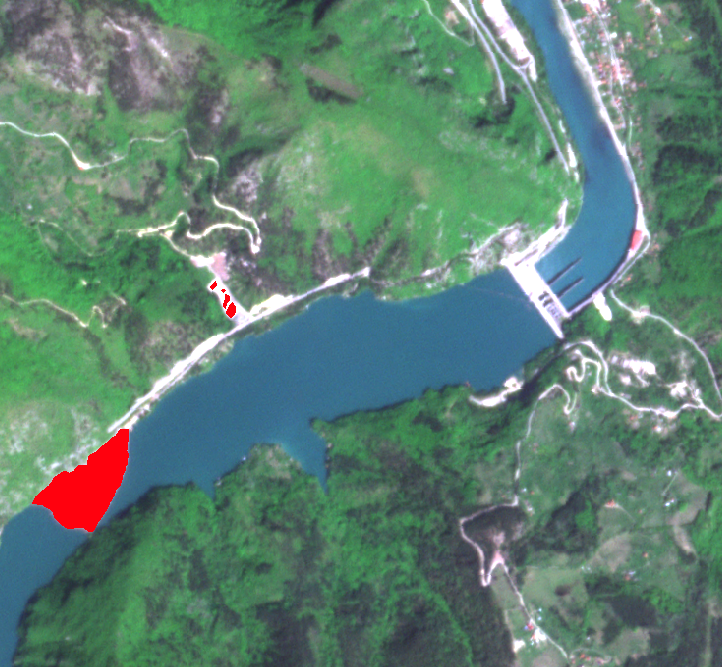
\includegraphics[width=0.45\linewidth]{drina-test}}
	\hspace{5pt}
	\subcaptionbox{A teszthalmaz annotációja az új modellel}{
		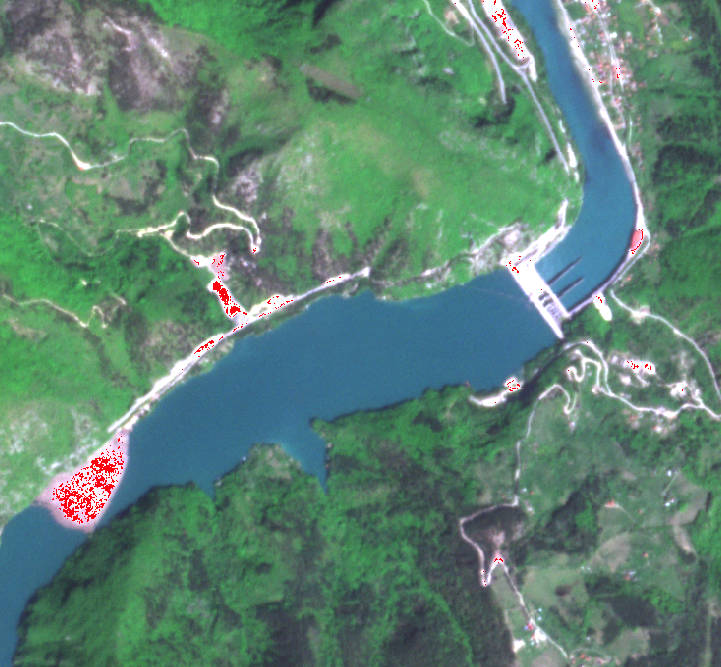
\includegraphics[width=0.45\linewidth]{drina-new}}
	\hspace{5pt}
	\subcaptionbox{A teszthalmaz annotációja az új modellel, PCA segítségével}{
		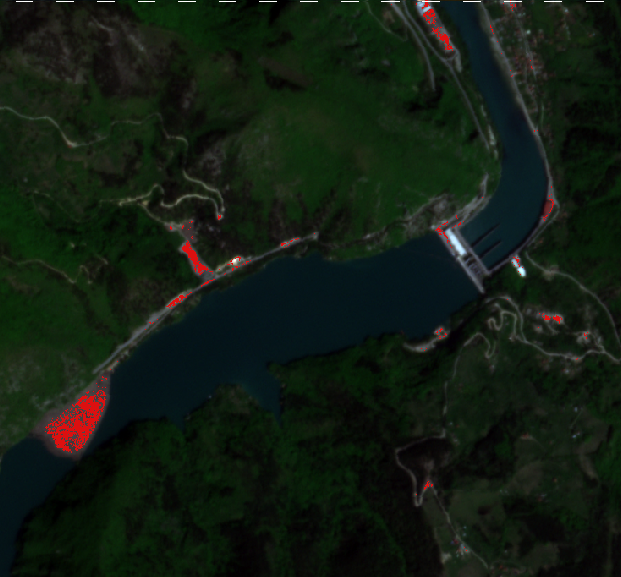
\includegraphics[width=0.45\linewidth]{drina-with-pca}}
	\caption{Az új modell összehasonlítása a PCA-val tanított modellel az egyik Drinai teszt felvételen. Felvétel dátuma: 2023-05-07}
	\label{fig:pca-vs-no-pca}
\end{figure}

A \ref{tab:pca-vs-no-pca} táblázatban összesítem a főkomponens analízis mutatóit. A táblázatból leolvasható, hogy míg a főkomponens analízis picivel nagyobb false positive aránnyal rendelkezik, egyben kisebb false negative aránnyal rendelkezik. Ráadásul a felvételeken készülő zajt sokkal jobban kezeli, amint a \ref{fig:classification-pca-vs-no-pca} ábrából is látható. A főkomponens analízissel betanított modell sokkal jobban tudta detektálni a vizet a folyón, mint a főkomponens analízis nélküi modell.

\begin{table}[H]
	\centering
	\begin{tabular}{ | p{0.33\textwidth} | p{0.33\textwidth} | }
		\hline
		\textbf{Mérés azonosító} & \textbf{PCA-val tanított modell átlagai (\%)} \\
		\hline \hline
		Comission Rate & 39.01 \\
		\hline
		Omission Rate & 65.00 \\
		\hline
		Match Rate & 34.99  \\
		\hline
        Extraction Rate & 65.25 \\
		\hline
	\end{tabular}
	\caption{A főkomponens analízissel betanított modell teljesítményének az átlagai}
	\label{tab:pca-vs-no-pca}
\end{table}

\begin{figure}[H]
	\centering
  \subcaptionbox{Drina műholdfelvétele}{
		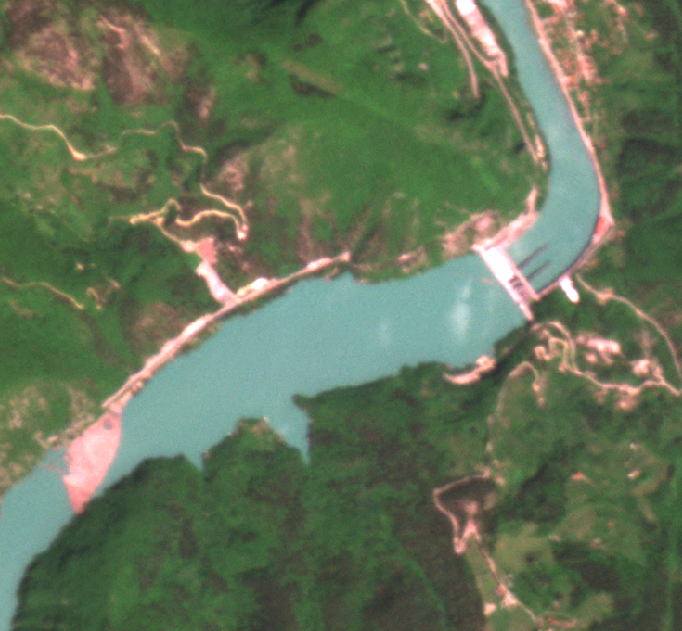
\includegraphics[width=0.45\linewidth]{drina20230521}}
	\hspace{5pt}
	\subcaptionbox{A PCA nélküli modell címkézése a Drinán}{
		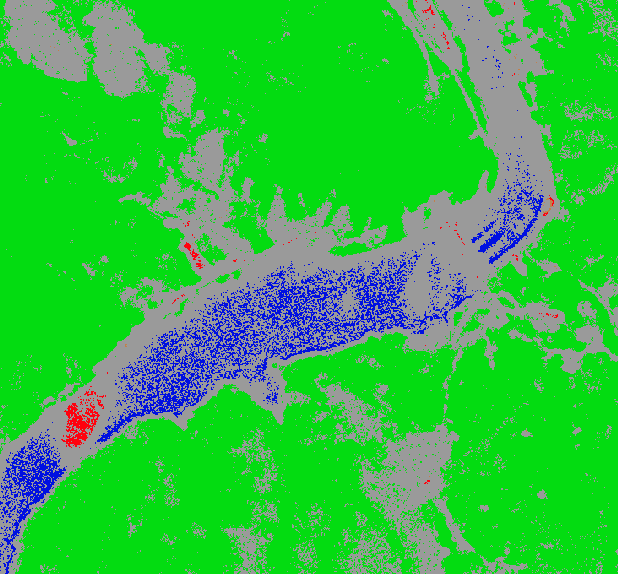
\includegraphics[width=0.45\linewidth]{drina-classification-no-pca}}
	\hspace{5pt}
	\subcaptionbox{A PCA-val betanított modell címkézése a Drinán}{
		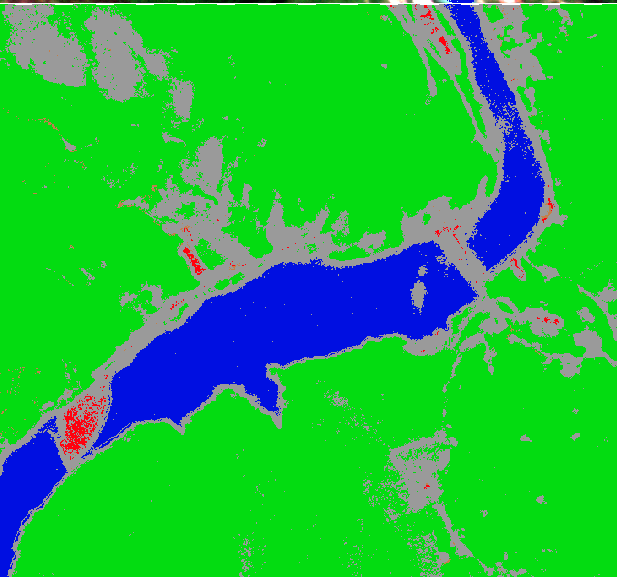
\includegraphics[width=0.45\linewidth]{drina-classification-with-pca}}
	\caption{A főkomponens analízissel betanított modell osztályozásának össszehasonlítása a PCA nélkül betanított modellel. Felvétel dátuma: 2023-05-21}
	\label{fig:classification-pca-vs-no-pca}
\end{figure}

\section{Vízmaszkolás}

Az egyik kihívás a hulladékdetektálásban a nagy lefedettségű területek feldolgozása. A kutatásunk célja a folyók közelében található hulladékkal szennyezett területeknek a detektálása, így a folyóktól távolabbi területeket érdemes kivágni a gyorsabb osztályozás érdekében. Az egyik hosszútávú cél az, hogy hosszabb folyószakaszokon is lehessen futtatni a Random Forest modellt, úgy, hogy az osztályozás elfogadható futási időn belül történjen meg.
\todo{hogy hivatkozhatok itt a laborban meglevő munkára, anélkül, hogy saját eredményként tűntessem fel?}  

\chapter{Megvalósítás és alkalmazás}
\label{ch:impl}

\subsection{A meglevő alkalmazások bővítése}
\label{ch:application-improvement}

\subsubsection {Az asztali alkalmazás bővítése}

A meglevő asztali alkalmazás alkalmas volt a tanítóadatok hatékony előállítására, de utólag nem lehetett visszanézni, hogy adott műholdfelvételhez milyen tanítóadatok tartoznak, illetve azt sem, hogy az adott tanítóadat hol volt mintavételezve. Az alkalmazás eredetileg egy CSV fájlba eltárolta az összes pixel spektrális értékeit és indexeit, és ezt lehetett használni tanításra. Ennek az volt a hátránya, hogy nehéz volt áttekinteni illetve kiegészíteni az adatokat. Ezért az asztali alkalmazást kiegészítettem ezzel a funkcionalitással, a tanítóadatok előállítása elmentésekor az alkalmazás létrehoz egy külön raszteres réteget is külön minden műholdfelvételhez, melyen látható, hogy mely területek voltak hozzáadva a tanítóadatok közé, így tetszőleges módon előállítható/ellenőrizhető a tanítóhalmaz.

\subsubsection {A szerveralkalmazás bővítése}

A szerveralkalmazás és webalkalmazás is bővítésre került: a szerveralkalmazás mostmár több modellt is le tud futtatni a letöltött műholdfelvételeken és ezeket külön tárolja. A webalkalmazás mostmár képes letölteni külön ezeket az eredményeket és több hulladékmaszkoló módszer eredményét is meg tudja jeleníteni, ennek köszönhetően ezeket egymással össze lehet könnyen hasonlítani valós tesztadatokon. 

\subsection{A Tiszta-Tisza alkalmazás}

A Tiszta-Tisza webalkalmazás \todo{melyik link kerüljön ide?} a PET Kupa által használt webalkalmazás, melynek az a célja, hogy egy olyan felületet biztosítson, ahol meglehet tekinteni a jelenleg ismert folyómentén található hulladéklerakókat, illetve akár a regisztrált felhasználók is be tudnak jelenteni ilyet. A PET Kupa megbízta az egyetemet azzal a feladattal, hogy ezt továbfejlessze, és a feladatok közé tartozott az is, hogy a Random Forest modell eredményeit integráljuk ebbe az alkalmazásba. Ezt a feladatot én vállaltam el.

Tekintve arra, hogy a Tiszta-Tisza térképén pontok vannak megjelenítve, a modell által detektált területeket is pontokkal jelöljük. Ehhez egy nagyobb terület közepére helyezünk el egy pontot. Előfordulhat olyan is, hogy a modell olyan képeket klasszifikál, melyek el vannak torzítva (például magas páratartalom miatt). Ilyenkor a false-positive-ok aránya lényegesen megnő. Ennek korrigálására a Tiszta-Tisza alkalmazásban a legutolsó három detektálást (legfeljebb 1 hónap különbséggel) veszem figyelembe és két kép közös metszetével döntöm el, hogy milyen területek kerülnek fel a térképre. A lépéseket a \ref{ch:intersection} fejezetben részletezem.

\subsection{Közös metszet}
\label{ch:intersection}

A már meglevő szervertől poligonok formájában, GeoJSON-ben \cite{rfc7946} lehet lekérni az adott napon detektált hulladékos területeket. így érdemes poligonok metszetében kigondolni a többségi szavazást. Jelöljük BUF(P,n)-vel egy multipoligon pufferét, ahol $$P \in \mathbb{P}$$ egy multipoligon, és n egy egész szám. Ekkor a többségi szavazást három képre a \ref{eq:voting} \todo{hasonló képleteket mások is ismernek fórumokban, de hivatalos forrással nem találkoztam} képlet szerint lehet alkalmazni. Ezután az elég nagy poligonok egy-egy belső pontját megválasztva megtudjuk jelölni a hulladéklerakókat.

\begin{equation}\label{eq:voting}
    Eredm\acute{e}ny \ multipoligon = \bigcup_{P_1 \in \mathbb{P}} \bigcup_{P_2 \in \mathbb{P}} BUF(BUF(P_1,n) \cap BUF(P_2,n),-n)
\end{equation}
\cleardoublepage

\chapter{Összefoglalás és eredmények}
\label{ch:sum}

\section{A kutatás során elért eredmények}

A dolgozatomban megvizsgáltam több módszert, amivel a korábbi modellben levő kihívásokat korrigáltam multispektrális Planetscope felvételeken. Előállítottam egy tanító adathalmazt, ami segítségével meg lehet vizsgálni több gépi tanulási módszert, illetve ki lehet próbálni több képfeldolgozási módszert. Megmutattam, hogy egy nagyobb tanító halmaz segítségével alacsonyabb false-positive arányokkal tudja a Random Forest modell detektálni a hulladékkal szennyezett területeket a teszthalmazban. Kiegészítettem az ELTE IK Térinformatikai laborban használt eszközöket arra, hogy hatékonyabban lehessen előkészíteni és megvizsgálni a különböző hulladékdetektálási módszereket. Megvizsgáltam a főkomponens analízis hatását a Random Forestre, és arra a következtetésre jutottam, hogy a modell láthatóan jobban kezelte PCA-val a többdimenziós felvételekben levő zajt, mint a PCA nélküli modell. Továbbá megnéztem, hogy miként teljesít a modell képnormalizálás, illetve vízmaszkolás mellett. Az utóbbi két módszert a laborban kutatják és fejlesztik a kollégáim. Bemutattam a módszer használhatóságát azzal, hogy a Tiszta-Tisza webalkalmazásába integráltam a Random Forest modell eredményeit, egyszerű poligonműveletek segítségével.

\section{A kutatás kihívásai}

A kutatás talán legnagyobb kihívása a tanító adatok megfelelő előállítása és a modellek validációja. A \ref{ch:waste-detection-methods} fejezetben bemutatott hulladékdetektálási módszerekben gyakori módszer volt egy magas felbontású műholdfelvétel használata validációra, vagy nagyon magas felbontású drónfelvételek használata a vizsgált területeken. A modell vizsgálata téli felvételeken is egy kihívás tekintve arra, hogy télen ritkábbak a megfelelő időjárás körülmények a nyári időszakokhoz képest. 

\section{További lépések}

A továbbiakban érdemes megvizsgálni akár személyesen, akár magas felbontású felvételekből a hulladékkal szennyezett területeket pontosabb validáció érdekében. Az adat-normalizálási módszereket is érdemes továbbvizsgálni, tekintve arra, hogy gyakori a zaj a műholdfelvételekben, így ilyen módszerek lényegesen növelhetik a modell megbízhatóságát. További lépésként javasolt akár más gépi tanulási módszereket is kipróbálni, illetve klasszikusabb térinformatikai eszközökkel is megközelíteni a hulladékdetektálás problémáját. Gépi tanulási irány esetén érdemes egy sokkal nagyobb adathalmazt előállítani, pontosabb adatvizsgálat mellett, így a modellek jobban tudják majd általánosítani az adatokat hulladékdetektálás céljából.

\cleardoublepage

% Acknowledgements (optional) - in case your thesis received funding or would like to express special thanks to someone
\chapter*{\acklabel}
\addcontentsline{toc}{chapter}{\acklabel}
Amennyiben a TDK projekted pénzügyi támogatást kapott egy projektből vagy az egyetemtől, jellemzően kötelező feltüntetni a dolgozatban is. A dolgozat elkészítéséhez segítséget nyújtó oktatók, hallgatótársak, kollégák felé is nyilvánítható külön köszönet.

% Appendices (optional) - useful for detailed information in long tables, many and/or large figures, etc.
\appendix
\chapter{Szimulációs eredmények}
\label{appx:simulation}

Lorem ipsum dolor sit amet, consectetur adipiscing elit. Pellentesque facilisis in nibh auctor molestie. Donec porta tortor mauris. Cras in lacus in purus ultricies blandit. Proin dolor erat, pulvinar posuere orci ac, eleifend ultrices libero. Donec elementum et elit a ullamcorper. Nunc tincidunt, lorem et consectetur tincidunt, ante sapien scelerisque neque, eu bibendum felis augue non est. Maecenas nibh arcu, ultrices et libero id, egestas tempus mauris. Etiam iaculis dui nec augue venenatis, fermentum posuere justo congue. Nullam sit amet porttitor sem, at porttitor augue. Proin bibendum justo at ornare efficitur. Donec tempor turpis ligula, vitae viverra felis finibus eu. Curabitur sed libero ac urna condimentum gravida. Donec tincidunt neque sit amet neque luctus auctor vel eget tortor. Integer dignissim, urna ut lobortis volutpat, justo nunc convallis diam, sit amet vulputate erat eros eu velit. Mauris porttitor dictum ante, commodo facilisis ex suscipit sed.

Sed egestas dapibus nisl, vitae fringilla justo. Donec eget condimentum lectus, molestie mattis nunc. Nulla ac faucibus dui. Nullam a congue erat. Ut accumsan sed sapien quis porttitor. Ut pellentesque, est ac posuere pulvinar, tortor mauris fermentum nulla, sit amet fringilla sapien sapien quis velit. Integer accumsan placerat lorem, eu aliquam urna consectetur eget. In ligula orci, dignissim sed consequat ac, porta at metus. Phasellus ipsum tellus, molestie ut lacus tempus, rutrum convallis elit. Suspendisse arcu orci, luctus vitae ultricies quis, bibendum sed elit. Vivamus at sem maximus leo placerat gravida semper vel mi. Etiam hendrerit sed massa ut lacinia. Morbi varius libero odio, sit amet auctor nunc interdum sit amet.

Aenean non mauris accumsan, rutrum nisi non, porttitor enim. Maecenas vel tortor ex. Proin vulputate tellus luctus egestas fermentum. In nec lobortis risus, sit amet tincidunt purus. Nam id turpis venenatis, vehicula nisl sed, ultricies nibh. Suspendisse in libero nec nisi tempor vestibulum. Integer eu dui congue enim venenatis lobortis. Donec sed elementum nunc. Nulla facilisi. Maecenas cursus id lorem et finibus. Sed fermentum molestie erat, nec tempor lorem facilisis cursus. In vel nulla id orci fringilla facilisis. Cras non bibendum odio, ac vestibulum ex. Donec turpis urna, tincidunt ut mi eu, finibus facilisis lorem. Praesent posuere nisl nec dui accumsan, sed interdum odio malesuada.
\cleardoublepage

% Bibliography (mandatory)
\phantomsection
\addcontentsline{toc}{chapter}{\biblabel}
\printbibliography[title=\biblabel]
\cleardoublepage

% List of figures (optional) - useful over 3-5 figures
\phantomsection
\addcontentsline{toc}{chapter}{\lstfigurelabel}
\listoffigures
\cleardoublepage

% List of tables (optional) - useful over 3-5 tables
\phantomsection
\addcontentsline{toc}{chapter}{\lsttablelabel}
\listoftables
\cleardoublepage

% List of algorithms
\phantomsection
\addcontentsline{toc}{chapter}{\lstalgorithmlabel}
\listofalgorithms
\cleardoublepage

% List of codes (optional) - useful over 3-5 code samples
\phantomsection
\addcontentsline{toc}{chapter}{\lstcodelabel}
\lstlistoflistings
\cleardoublepage

% List of symbols (optional)
%\printnomenclature

\end{document}
